\documentclass{llncs}
\usepackage{graphicx}
\usepackage{amsmath}
\usepackage{listings}
\usepackage{tikz}
\usepackage{epstopdf}
\usepackage{multirow}
\usepackage{todonotes}



\title{Your Awesome Project Title}

\author{Firstname Lastname\inst{1}}
\institute{	University of L\"ubeck, Germany\\
	\email{firstname.lastname@student.uni-luebeck.de}}


\begin{document}
\maketitle


\begin{abstract}
A short description of your project (150-250 words).

This document is intended as a guide to structure your project and to help you to document your work in a paper structure.

\end{abstract}



\section{Motivation}
\todo[inline]{Know what you want to do and why that is interesting (maybe with bullet points). But do not write this section until you know what you actually have done so that the motivation fits your work.}

To generate this pdf, you need a latex implementation. I recommend TeXstudio, but there are others. For your references (the .bib file) jabref is the only helpful editor I have used, but most publishers provide helpful bibtex references on their web sites.
Refer to sections like this: Section~\ref{sec:background} and to references like this: Ristenpart et al.~\cite{Ristenpart_hey}. 


We will stick to the following timeline:

\begin{itemize}
	\item 13.11.: Project goals and outline defined
	\item 20.11.: Related work as well as detailed outline identified and described in report
	\item 4.12.: At least 1/3 of your anticipated work should be completed and documented
	\item 18.12.: At least 2/3 of your anticipated work should be completed and documented
	\item 15.1.: All of your anticipated work should be completed and documented, including results and outcomes
	\item 22.1. : Test presentation ready 
	\item from 25.1.: Presentation of your project in class.
	\item from 12.2.: Submission of final version of your report.
\end{itemize}

\section{Background}\label{sec:background}
\todo[inline]{You should find and describe related work early on. Know what other people have done.}

\section{Work Description}
Here you describe the work you have performed, problems you have solved and methods you have used. There is a fine balance between brevity and conciseness and ensuring that other people, if investing the time, would be able to reproduce your results given this description.



\section{Results}
\todo[inline]{here you will present and discuss your outcomes: implementation results or measurements or other project outcomes}

\subsection{Subsection 1}
\begin{figure*}[t!]
	\centering
	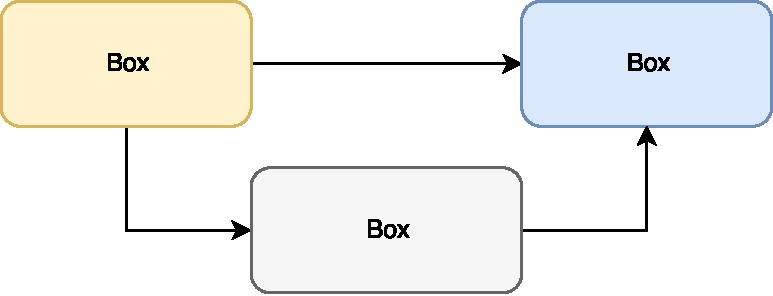
\includegraphics[width=.99\linewidth]{images/examplepicture}
	\caption{A picture that shows boxes and arrows.}
	\label{fig:examplepicture}
\end{figure*}


Figure \ref{fig:examplepicture} contains an image.

\section{Conclusion}
\todo[inline]{TBD last}

\bibliographystyle{alpha}
%\bibliographystyle{splncs03}
\bibliography{references}
\end{document}
